
%% bare_jrnl.tex
%% V1.4
%% 2012/12/27
%% by Michael Shell
%% see http://www.michaelshell.org/
%% for current contact information.
%%
%% This is a skeleton file demonstrating the use of IEEEtran.cls
%% (requires IEEEtran.cls version 1.8 or later) with an IEEE journal paper.
%%
%% Support sites:
%% http://www.michaelshell.org/tex/ieeetran/
%% http://www.ctan.org/tex-archive/macros/latex/contrib/IEEEtran/
%% and
%% http://www.ieee.org/



%%*************************************************************************
%% Legal Notice:
%% This code is offered as-is without any warranty either expressed or
%% implied; without even the implied warranty of MERCHANTABILITY or
%% FITNESS FOR A PARTICULAR PURPOSE! 
%% User assumes all risk.
%% In no event shall IEEE or any contributor to this code be liable for
%% any damages or losses, including, but not limited to, incidental,
%% consequential, or any other damages, resulting from the use or misuse
%% of any information contained here.
%%
%% All comments are the opinions of their respective authors and are not
%% necessarily endorsed by the IEEE.
%%
%% This work is distributed under the LaTeX Project Public License (LPPL)
%% ( http://www.latex-project.org/ ) version 1.3, and may be freely used,
%% distributed and modified. A copy of the LPPL, version 1.3, is included
%% in the base LaTeX documentation of all distributions of LaTeX released
%% 2003/12/01 or later.
%% Retain all contribution notices and credits.
%% ** Modified files should be clearly indicated as such, including  **
%% ** renaming them and changing author support contact information. **
%%
%% File list of work: IEEEtran.cls, IEEEtran_HOWTO.pdf, bare_adv.tex,
%%                    bare_conf.tex, bare_jrnl.tex, bare_jrnl_compsoc.tex,
%%                    bare_jrnl_transmag.tex
%%*************************************************************************
%
\documentclass[11pt,journal]{IEEEtran}
\usepackage{ifpdf}
\usepackage{cite}
\usepackage[pdftex]{graphicx}
\graphicspath{{./img/}}
\DeclareGraphicsExtensions{.png,.jpg}
\usepackage[cmex10]{amsmath}
\usepackage{array}
\usepackage[caption=false,font=footnotesize]{subfig}
\usepackage{fixltx2e}
\usepackage{stfloats}
\usepackage{url}

% correct bad hyphenation here
%\hyphenation{op-tical net-works semi-conduc-tor}

\begin{document}
\title{Ocelot: Minimal Bounding Planar Quadruped}
\author{Sam Calisch,~\IEEEmembership{Center for Bits and Atoms,}
        Will Langford,~\IEEEmembership{Center for Bits and Atoms}
%\thanks{Thanks to Sangbae Kim, Matt Haberland, Neil Gershenfeld.}%
}
\markboth{2.S997, Biomimetics, Biomechanics, and Bio-inspired Robots, Fall~2013}%
{Hey there.}
\IEEEspecialpapernotice{Invidual Report, Calisch}


\maketitle
%\begin{abstract}
%The abstract goes here.
%\end{abstract}
\IEEEpeerreviewmaketitle



%Purpose: 
%The purpose of the individual reports is to 
%1) document the work done on the final project and 
%2) to encourage knowledge transfer among teammates. 
%Consequently, the writing will differ from and be more detailed than the text of the exhibition posters, as 
%their purpose was to present the work to the public. Also, regardless of how final project work was 
%distributed within teams, all team members should have broad understanding of all aspects of the project. 
%Content: 
%The report should include, but need not be limited to, the following sections: 
%0. Title 
%1. Introduction � motivation and background information 
%2. Project description 
%2.1. Computational experiment 
%2.1.1. Methods � model, schematic, optimization/computer experiment setup 
%2.1.2. Results 
%2.2. Physical experiment 
%2.2.1. Methods � Robot design, robot experimental setup 
%2.2.2. Results 
%3. Discussion � What went well? How could things have been improved? What did you learn? How 
%could the project be extended in the future? 
%4. Conclusion 
%While all sections are required, it is fine to include more detail in the sections about the work you did. 
%The report should include enough information to fill at least 4 single-spaced pages with 12pt font, 
%including figures. Note: use of smaller fonts (10pt, 11pt) is acceptable if they are easily readable, and you 
%are welcome (indeed encouraged) to use a two-column format similar to many conference publications 
%(i.e. IEEE). 
%Grade: 
%The individual report is 15% of your final grade. Roughly equal weight will be given to your motivation, 
%simulation experiment, and hardware experiment. Because comparable emphasis is placed on motivation, 
%it is important to demonstrate in your introduction and discussion the greater significance of your 
%investigation (e.g. explain why the questions you attempted to answer have scientific/engineering merit).


\section{Introduction}
%motivation and background information
\IEEEPARstart{B}{iological} quadrupeds use a remarkable variety of gaits to move around, including trotting, cantering, galloping, pacing, pronking, and bounding.  In some of these gaits, certain pairs of legs are used in synchrony:  trotting joins together the diagonal legs, pacing links lateral ones, and bounding pairs anteroposterior ones \cite{mitleg}.  This fact has been used extensively in biomechanics literature to simplify gait analysis and generation, perhaps most notably by \cite{raibert} to relate quadrupedal and bipedal gaits.  Many analyses use the anteroposterior pairing to simplify their study.  That is, instead of studying a full quadruped in three dimensions, the authors flatten the quadruped into the sagittal plane.  These \emph{planar quadruped} models can tell a great deal about the performance of true quadrupeds; for instance, \cite{haynes} builds a simulation of two SLIP legs joined by a compliant spine and \cite{qu} relates joint and spine stiffnesses to gait self-stability for this model.

This flattening can also be used to simplify the construction of robots by reducing the required degrees of freedom to achieve these gaits.  A physical planar quadruped has its two front and two rear legs linked and driven by a single motor each.  This linking means the robot has no hope of trotting or pacing, but it could still bound.  Despite this significant simplification, we could find only one true example in the literature of a robot like this: \cite{leeser} famously built a constrained planar quadruped to study the effect of an articulated spine on locomotion.  Many quadrupedal robots can operate in a planar mode (e.g. \cite{bdcheetah}, \cite{nessi}, \cite{pusey}, \cite{khoramshahi}), but since they have actuators for each of four legs, they do not enjoy the simplicity of a true planar quadruped.  The robot in \cite{ho} is similar in spirit to a true planar quadruped, but it operates in a different regime of leg amplitude and frequency.

We took this as an opportunity to exploit the simplicity of planar quadrupeds to create the lowest degree-of-freedom bounding robot possible with controllable speed capable of more than one body length per second without planar constraint.  

A first guess at such a robot might have front and rear legs that extend and change angle relative to the body.  Examining bounding in biological quadrupeds suggests this might be redundant.  Indeed, when it bounds, the cheetah seems use only three main degrees of freedom: rear leg extension, front leg extension, and an angle change between the front and rear legs.  That is, individual angle control of the legs is not necessary.  This insight lead us to a three degree-of-freedom planar quadruped, where the angle between front and rear legs is controlled by an articulated spine.

In what follows, we first survey our progress in simulating the behavior of planar quadrupeds of this type.  Then, we outline our work designing and prototyping a physical bounding robot named Ocelot.  Finally, we discuss the general implications to bounding and bounding robots.

%%%
\section{Simulation}
\begin{figure}[!t]
\centering
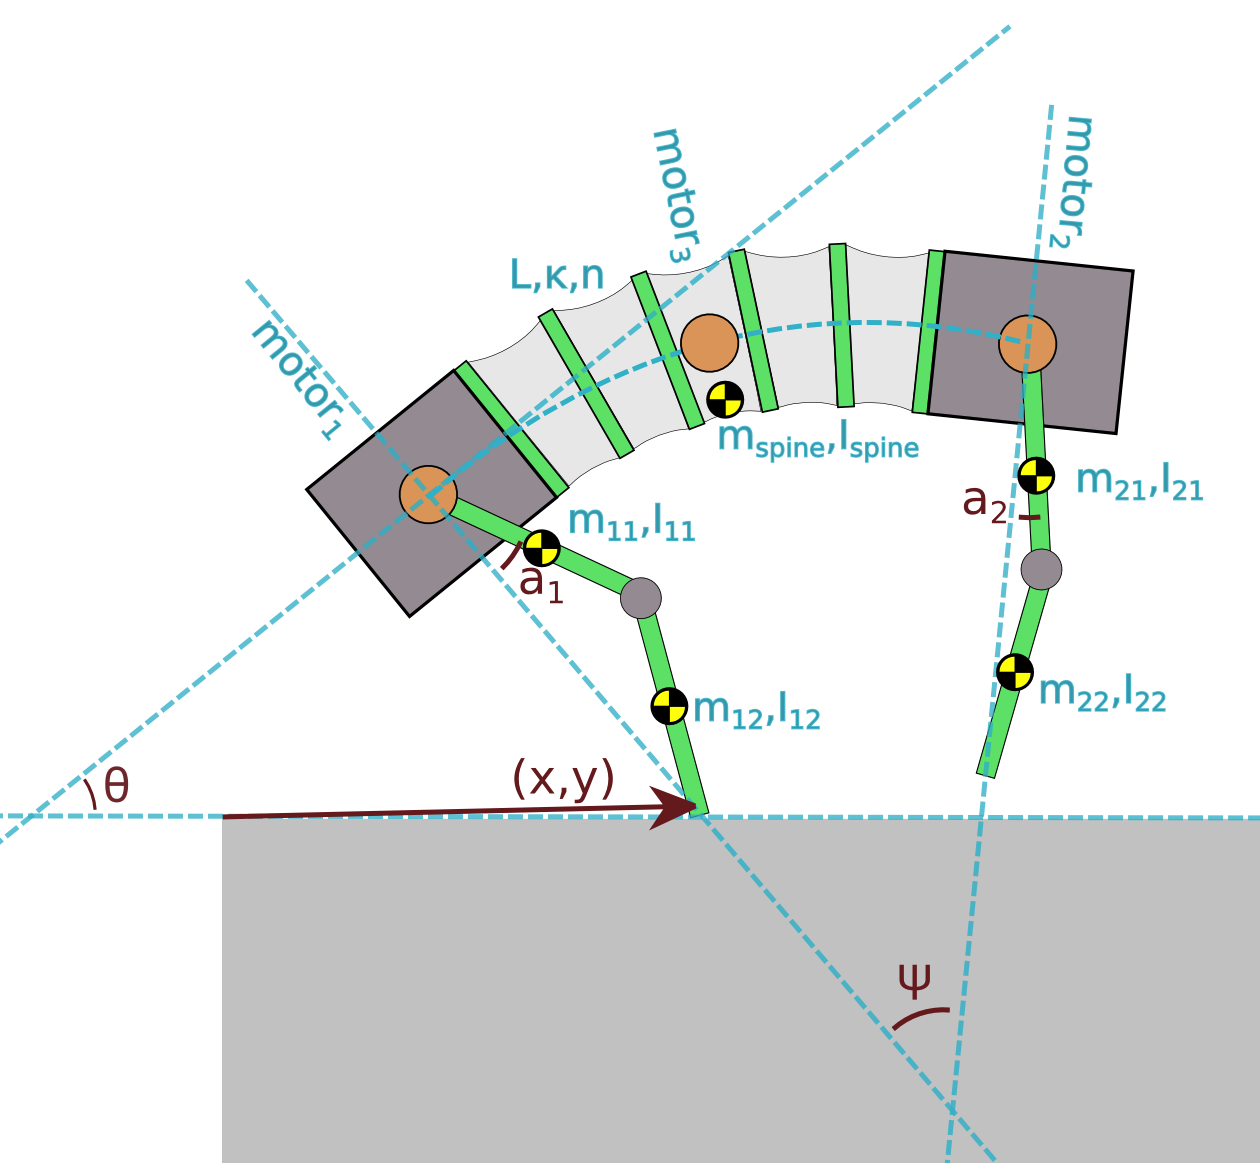
\includegraphics[width=3.in]{diagram-1a}
\caption{Simulation schematic}
\label{fig_sim}
\end{figure}

\subsection{Methods}
%� model, schematic, optimization/computer experiment setup
\subsubsection{Lagrangian dynamics}
Our first task of study was to build a simulation of bounding dynamics that could accommodate the full design space we want to consider for our physical prototype.  To simplify implementation and lower computational cost, we only consider sagittal plane motion.  Obviously, a physical robot has more degrees of freedom than this allows (even if it is designed to stay in a plane), but we assume we will be able to mitigate yaw and roll modes with appropriate design of the contacting surfaces and mass distribution.

The simulated robot has three degrees of freedom, shown in Figure \ref{fig_sim}.  First, front and rear legs can each extend and contract along lines from the hip and shoulder.  These lines are usually nearly perpendicular to the central axis of the robot, but the relative angle is adjustable.  This extension/contraction is given by angles $a_1$ and $a_2$ produced by the motors.  The third degree of freedom is specified by the subtended angle $\psi$ of the articulated spine.  The number of links in the spine, as well as as the overall length and an optional restorative spring can be adjusted. The spine's center of mass and moment of inertia is calculated symbolically in the generalized coordinates.  The internal coordinates were chosen to correspond to the motor encoders to within a constant gearing factor.  This is obvious for the legs, but worth noting that for tendon, gear, or pulley actuation of the spine, this gearing factor can be readily derived based on geometry.  We can specify the rigid body transformation of the robot in the plane with three coordinates, $x, y, \theta$, measured from the origin to rear foot.

The simulation uses four integration phases: both feet in contact, rear foot in contact only, front foot in contact only, and full flight.  To switch between these phases, we implemented four event conditions based on front foot height, rear foot height, front foot vertical constraint force, and rear foot vertical constraint force.  For instance, if the rear foot is in contact, we watch for zeros in the vertical constraint force there, switching to front contact only or full flight (depending on the condition of the front foot).  To constraint horizontal motion, the feet are assumed to be perfectly sticky.  Thus, when a foot is in contact, the ground exerts a horizontal constraint force to keep it in place.  

Each leg and spine link has a center of mass along its length, as well as a specified rotational inertia.  Motors (modeled as point masses) are positioned at the hip, shoulder, and along the spine.  From this full description we formulated the Lagrangian dynamics problem and derived the equations of motion for the system.  Using these with initial conditions for all coordinates and specified motor torque control laws, we can create trajectories for the robot through space using Matlab's \texttt{ode45} numerical integration routine.

\subsubsection{Optimization}
This simulation produced physical results, but finding appropriate control laws for a desired trajectory is a difficult task to do by hand.  To this end, we wrapped the simulation in an outer optimization loop using Matlab's \texttt{fmincon}.  Using nested functions, we can force \texttt{fmincon} to evaluate the expensive simulation just once when computing both the objective and the constraints.  We implemented several schemes for specifying control laws with the optimization's decision variable; we describe them below.

First we tried a multiple shooting scheme, dividing the control signals into phases corresponding to the phases of the simulation.  Each phase was allotted three values over which the control signals were interpolated.  The decision variable also contained the transition times between phases, which we constrain to correspond to the event times from the simulation.  We found a simple hopping trajectory by hand that was nearly periodic to use as a starting point.  Periodicity in all generalized coordinates except $x$ was enforced as an optimization constraint, and the objective function rewarded horizontal travel.

The second scheme was considerably simpler and used a heuristic we had seen work well to control the physical robot.  We assume the coordinate profile each motor over a period looks like a ramp up to a maximum value, time spent at the maximum, a ramp down to a minimum value, and time spent at the minimum value.  We also assume the front and rear legs are $180^\circ$ out of phase, and the spine has a specified phase shift from the legs (usually $90^\circ$).  We further decided to smooth these piecewise linear signals to produce smoothly varying signals at the controller frequency so that the PD controller would have better behavior.  With these assumptions, the decision variable contained maximum and minimum angle values for the legs and spine, as well as fractions of the period spent ramping and holding.


\subsection{Results}
\begin{figure}[!t]
\centering
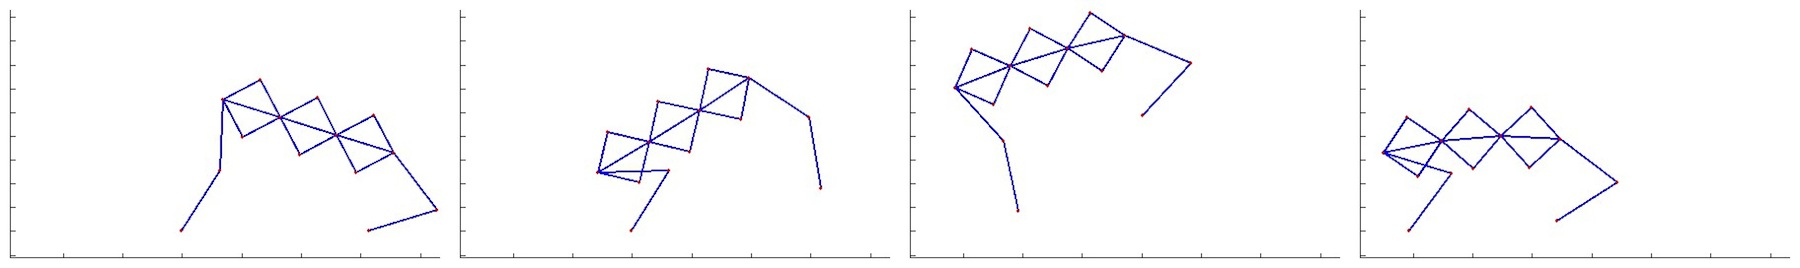
\includegraphics[width=3.5in]{sim-grid}
\caption{Simulated bounding}
\label{sim_bound}
\end{figure}


\begin{figure}[!t]
\centering
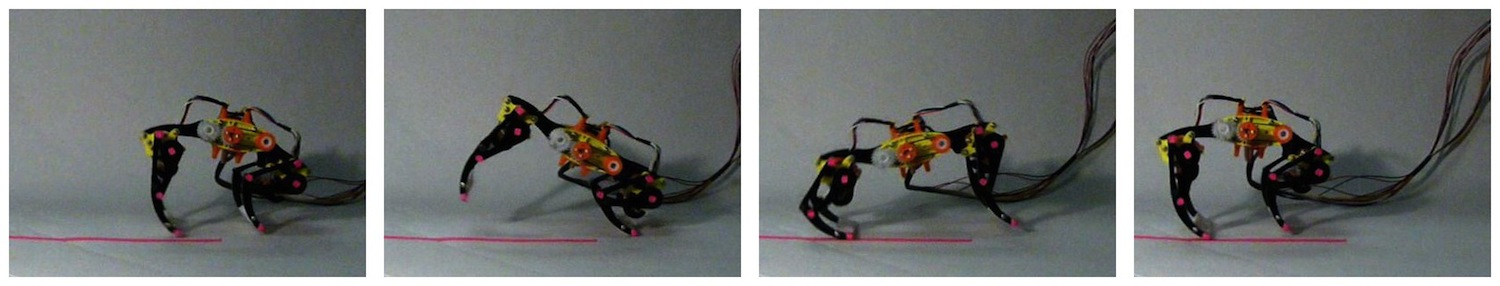
\includegraphics[width=3.5in]{grida}
\caption{Bounding gait.}
\label{physical_bound}
\end{figure}

The first optimization scheme was designed to make few assumptions about the control signals.  By dividing the time domain into meaningful portions (the phases) that could be easily stitched together, we could represent gaits with relatively few interpolation values.  Despite these advantages, the decision variable contained roughly 50 entries.  For a problem with so many local minima, this proved too many dimensions to reasonably extract efficient gaits with Matlab's sequential quadratic programming or interior point algorithms.

With the same objective functions as the first scheme, the second scheme made some progress from a good initial guess towards gaits that moved horizontally.  Despite the initial guess being nearly periodic, optimization iterations consistently violated the periodicity constraint.  

Both schemes were plagued by some limitations of the underlying simulation.  First, observation of our physical prototype suggests that some slipping of the foot is a fundamental part of a stable bounding gait for this robot.  The stickiness assumption of the simulation turned out to be more restrictive than initially assumed.

This effect was compounded by missed events in \texttt{ode45}.  Often, the robot's feet fall through the floor as the integrator misses a root in the vertical position function.  Conversely, when the integrator misses a takeoff event, the robot is pulled down by a foot instead of taking off into flight.  These missed events are not smooth in the decision variable, and hence cause the optimization algorithm serious problems.

Despite these limitations, these experiments showed that the torque output of the motors was sufficient to generate the accelerations of the robot necessary for bounding.  Further, when forming hypotheses about the speed controller (discussed below), the simulation showed that the sign of the spine amplitude could control the direction of horizontal travel of the robot.


%%%
\section{Physical Experiment}
%Robot design, robot experimental setup 

\subsection{Methods}
\begin{figure}[!t]
\centering
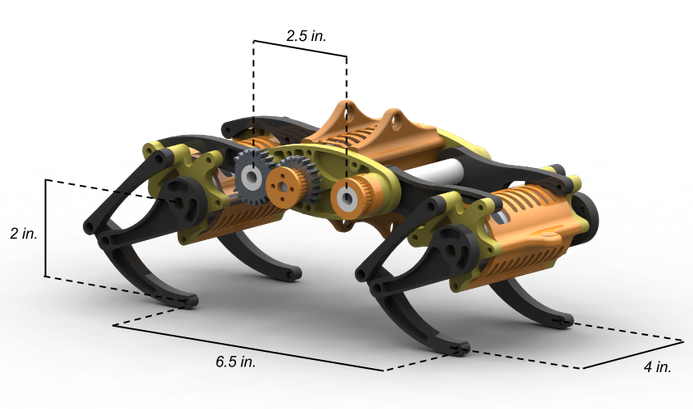
\includegraphics[width=3.5in]{render}
\caption{Mechanical model of Ocelot}
\label{speed}
\end{figure}
As described above, Ocelot, our planar quadrupedal robot, had rigidly mounted front and rear legs.  The extension of each leg was controlled by a single motor each.  The motor drives the femur segment on one side of the robot, and the legs are tied together with segments spanning the tibial region.  We found no evidence for changing the mounting angle of the leg relative to the body, so we left it at $90^\circ$.  

To simplify the design, we used only three spine segments (originally, we though to use more).  The spine motor is attached to the central section and it uses a gear to drive one spine joint and a pulley to drive the other.  The gear reverses the drive direction on one joint, producing the curling motion that was desired.  Initially, we installed an elastic band along the spine to assist the spine motor, but we determined this was not necessary and eventually removed it to save mass.

Ocelot's size was determined by considering the maximum force that each leg could exert. Using a rule of thumb that the maximum acceleration required for this gait is 2.5$g$, and the motor's supplied torque of 1.5 $N\cdot m$, we calculated that the leg segments should be no longer than 3 inches.  To be safe, the leg segments were set to be 2 inches long, and the rest of the robot's dimensions were determined proportionally.

Ocelot was fabricated primarily on a Shopbot Desktop CNC router out of high-density polyethylene (HDPE) and Delrin stock.  The timing belt pulleys, motor cases, and feet were printed on a Makerbot Replicator II 3D printer, and the gears were cut on an OMAX waterjet abrasive machining center.  The drive side femurs were original milled from Delrin, but were replaced with aluminum versions machined on a Hurco VM10U high speed machining center, in order to eliminate the separate motor shaft mounting plate.

The three motors are commanded by one VNH5019 motor driver each, which in turn are controlled by an MBED microcontroller.  An external power supply gives 18 $V$, capped at 10 $A$.  Ocelot is given position trajectories for each motor (an example is shown in the left of Figure \ref{traj}) and a PD position control loop calculates required torques at 500 Hz.  The torques are then supplied by a calibrated current control loop.

The robot is tethered with three segments of ribbon cable (one for each motor controller), and heavier lines for power.  A small milled circuit board houses the quick interconnect components for ease of travel.

\begin{figure}[!t]
\centering
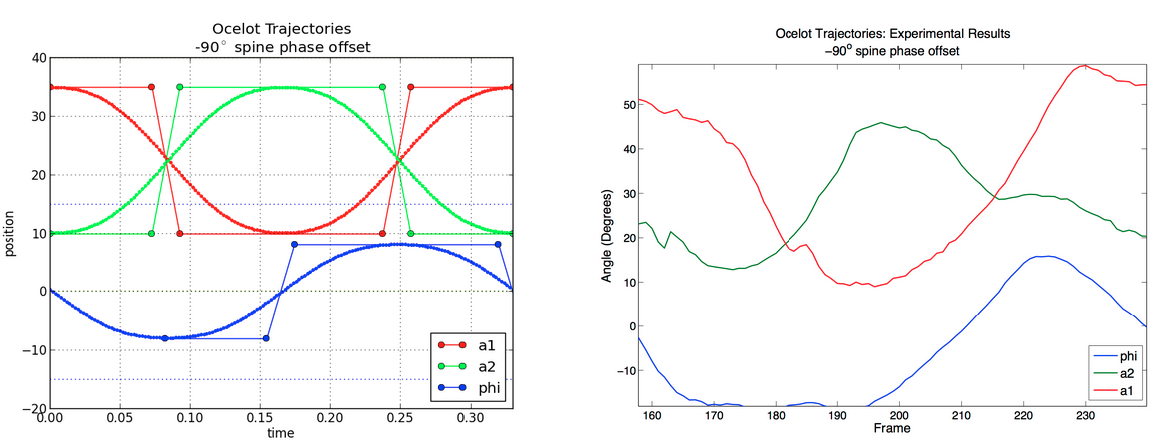
\includegraphics[width=3.in]{trajectories}
\caption{Input trajectories (left), and tracked joint trajectories (right)}
\label{traj}
\end{figure}

%%%
\subsection{Results}


The final robot prototype weighed 800 $g$, well within the capabilities of the motors to produce accelerations of 2.5$\cdot g$ $m/s^2$.  To achieve this weight, we removed or replaced all unnecessary components, including the motor gearbox covers and the motor shaft coupling.

Developing trajectories that reliably produced a bounding gait was initially a challenge.  Performance was highly dependent on the interface between the foot and the ground.  We tried foot coverings of VHB tape, adhesive sandpaper, and sorbothane, but eventually settled on using the naked PLA foot on a foam core ground covered in heavyweight paper. Once we standardized this interface, we could produce more reliable results.  Another confounding factor was the range of angles of the joints, as the linkages work well over a range smaller than their full travel.  We installed bumpers to limit the minimum angle of the legs, and avoided sending commands that extended the legs too much.  With these two adjustments, it was much easier to test hypotheses and develop a gait model.  An example of the commanded positions is shown on the left of Figure \ref{traj}.  As described in the simulation section, the signals are generated from maximum and minimum values, as well as time periods for ramping and holding.  The signals are then smoothed before being given the the PD controller.

Part of this development included verifying that the robot was performing as commanded.  We applied markers to key points on the robot and extracted the joint positions using high speed video tracking.  A comparison of commanded and measured positions is shown in Figure \ref{traj}.  The two correspond except at moments of high force application, as expected.

Moments in the gait required high current ($>6 A$), but these currents could (and did) destroy motors if supplied for an extended time ($\ge1 s$).  To remedy this, we used a digital smoothing filter in the control loop to extract a stable current reading to be used in safety measurements.  If this ever exceeds a large value (8 $A$), we set the PWM duty cycle to zero as a safety precaution.  Further, we keep track of the number of time steps at which the averaged current is above a less extreme, but still high current (5 $A$).  If this count exceeds the equivalent of .8 $s$, we shut down the robot completely.

With reasonably stable gait trajectories established, we created a speed controller to determine the range of possible speeds for Ocelot.  Based on observation, the amplitude of the spine signal seemed to correspond to speed.  Figure \ref{speed} shows that this is the case: as we increase spine amplitude from 8$^\circ$ to 20$^\circ$, Ocelot's average horizontal speed increases from .5 to 1.5 body lengths per second.  Further, by using a negative amplitude, Ocelot runs in the opposite direction.  For these trials, stride period is held constant as spine amplitude varies.  Likely this produces suboptimal speed at some values of spine amplitude, as realized through foot slippage, but we still have a speed controller with sufficient range.

\begin{figure}[!t]
\centering
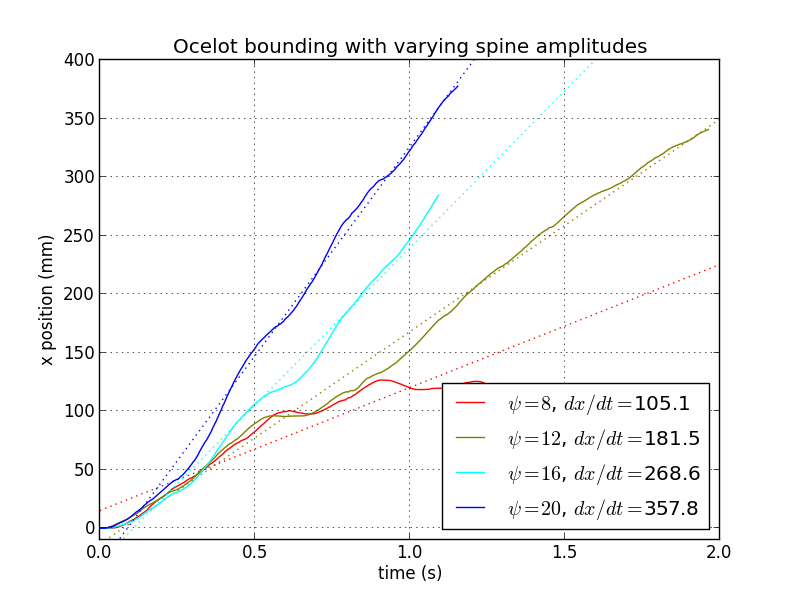
\includegraphics[width=3.2in]{speed-plot}
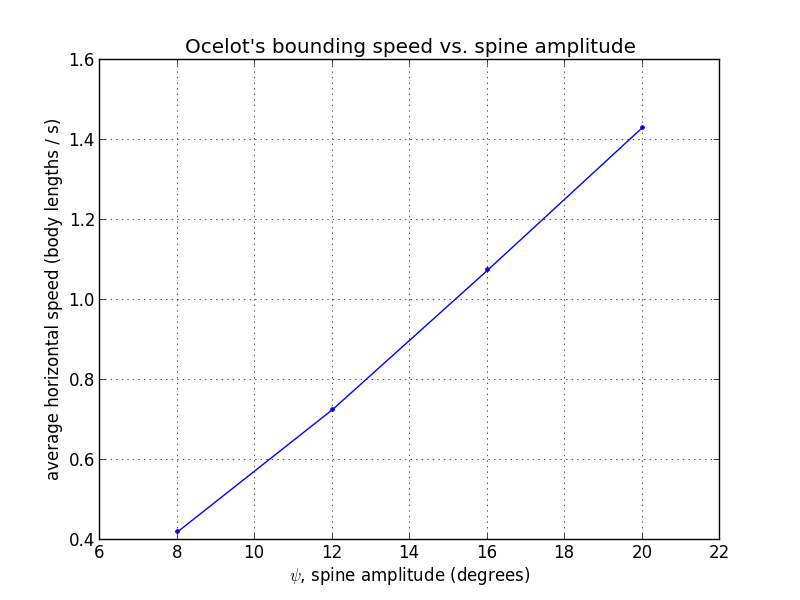
\includegraphics[width=3.2in]{speed-plot-2}
\caption{Ocelot's speed controller, varying spine amplitude offers control of horizontal speed.}
\label{speed}
\end{figure}

%%%
\section{Discussion}
%� What went well? How could things have been improved? What did you learn? How could the project be extended in the future?

Overall, this experiment achieved the goals laid out in the introduction.  The choices of fabrication processes was a big part of this success.  Because many parts were milled, as opposed to 3D printed, we could iterate quickly if a part did not perform as designed.  Another feature adding to this success was the ability of motors and encoders to do effective impedance control.  In the end, this simplified the robot considerably as we had planned to use an elastic band in the spine but found we could implement a virtual spring with great results.

Not everything worked so well, however.  It was exciting to be able to implement all features of the robot in a kinematic simulation, but the total amount of knowledge extracted from this simulation was disappointing.  The simplified friction model and the events missed by the integrator created enough nonphysical (and non-smooth) phenomena that it proved difficult to get the optimization routines to return useful information.  We could improve these errors by writing a physical model of friction (at a computational cost), as well as implementing more robust detection of gait phase transitions.  Further improvements to the simulations accuracy could be made by modeling the backlash in the robot mechanics (particularly the spine).

Another area for improvement is in the leg design.  The combination of shoulder bolts with Delrin proved problematic for several reasons.  First, the Delrin consistently measured .015" thicker than its .25" specification, and the shoulder bolts are designed around .25" material.  To improve, we could simply mill the Delrin to .25" before cutting the parts.  Second, in plastic the shoulder bolts are difficult to install perfectly perpendicularly to the surface.  This causes the legs to bind up frustratingly often. This problem could be fixed by using threaded inserts, as opposed to threading directly into the delrin.  Finally, as the legs are only driven from one side, the accumulated slop through the kinematic chain causes some lag between right and left.  An improved design would tie the legs together at two points (the ankle and the knee) instead of just one.

There are many ways Ocelot could be extended in the future.  First and most importantly, the improvements to the simulation mentioned above would allow considerably more testing of gaits and design changes.  It is likely that higher speeds and better efficiencies would come from these studies.  Second, because Ocelot weighs only 800$g$, it could be possible to create self-supported version with a lithium polymer battery.  Without the tether, we could use our speed controller to create a remote controlled quadruped.  Third, an interesting project could be to fully characterize the relationship between spine amplitude, horizontal speed, and stride period.  As a result, we might be able to write a speed controller which varies both spine amplitude and stride period as a function of desired speed.  These gaits would likely be more efficient, due to reduced foot slippage and other losses.


%%%
\section{Conclusion}
This project aimed to show that a robot can achieve high-performance bounding ($>1$ body length per second) with just three degrees of freedom, in order to reduce cost and complexity.  Our robot, Ocelot, easily reached parameter-controlled speeds between .5 and 1.5 body lengths per second, cost roughly \$200 in parts, and was fabricated in a single day. By this measure, the project was successful, but as detailed above there is considerable room for improvement.  Given the complexity of legged locomotion in general, however, we were thrilled with these results and hope this work can lower the barrier to entry for experiments with bounding robots.

%%%
\section*{Acknowledgment}
I would like to Sangbae Kim and Matt Haberland for teaching a thought-provoking and exciting class.  I would also like to thank Neil Gershenfeld for providing facilities and resources for fabrication and testing.  Finally, I would like to thank my partner, Will Langford, for his uncanny productivity and love of milled polyethylene.  

\ifCLASSOPTIONcaptionsoff
  \newpage
\fi

\begin{thebibliography}{1}
\bibitem{bdcheetah}
Boston Dynamics. \emph{CHEETAH - Fastest Legged Robot}. \url{http://www.bostondynamics.com/robot_cheetah.html}
\bibitem{qu}
Cao, Qu and Ioannis Poulakakis. \emph{Self-stable Bounding with a Flexible Torso}\url{http://udel.edu/~caoqu/publications/cao_poulakakis_AMAM13.pdf}
\bibitem{haynes}
Haynes et al, \emph{Dynamic Bounding with a Passive Compliant Spine}.
\bibitem{ho}
Ho, Thanhtam, Sunghac Choi, Sangyoon Lee. \emph{Piezoelectrically Actuated Biomimetic Self-Contained Quadruped Bounding Robot}
\bibitem{khoramshahi}
Khoramshahi et al, \emph{Bene�ts of an Active Spine Supported Bounding Locomotion With a Small Compliant Quadruped Robot}.
\bibitem{leeser}
Leeser, \emph{Locomotion Experiments on a Planar Quadruped Robot with Articulated Spine}.
\bibitem{mitleg}
MIT Leg Laboratory. \emph{Quadruped (1984-1987)}. \url{www.ai.mit.edu/projects/leglab/robots/quadruped/quadruped.htm}
\bibitem{nessi}
Nessi, Mateo. \emph{Design of a compliant spine for the Locomorph quadruped robot}. \url{http://biorob.epfl.ch/files/content/sites/biorob/files/public/Rico/final_presentation_matteo_nessi.pdf}
\bibitem{raibert}
Raibert, M.H. \emph{Trotting, pacing and bounding by a quadruped robot}.  J Biomech.  1990:23 Suppl 1:79-98
\bibitem{pouya}
Pouya, et al., \emph{Role of Spine Compliance and Actuation in the Bounding Performance of Quadrupeds}.
\bibitem{pusey}
Pusey et al., \emph{Free-standing Leaping Experiments with a Power-Autonomous Elastic-Spined Quadruped}. 

\end{thebibliography}

\begin{figure}[!t]
\centering
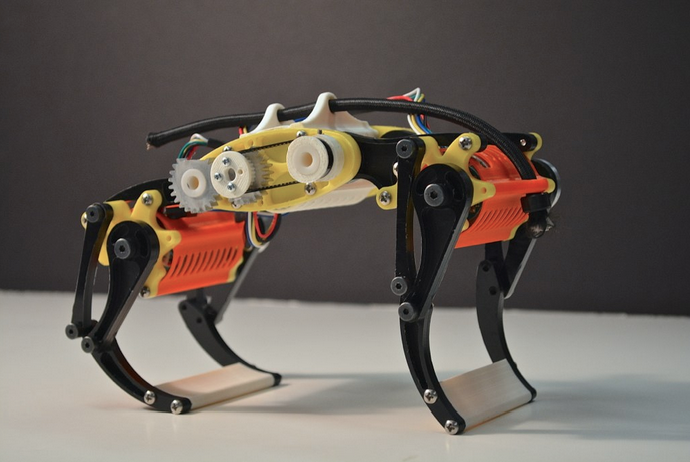
\includegraphics[width=3.5in]{ocelot}
\label{ocelot}
\end{figure}

\end{document}


